\documentclass[8pt,aspectratio=169]{beamer}
\usetheme{Madrid}
\usepackage{graphicx}
\usepackage{booktabs}
\usepackage{adjustbox}
\usepackage{multicol}
\usepackage{amsmath}
\usepackage{amssymb}
\usepackage{tikz}
\usepackage{hyperref}
\usepackage{algorithm}
\usepackage{algorithmic}
\usepackage{colortbl}
\usepackage{pgfplots}
\pgfplotsset{compat=1.18}

% TikZ libraries for comics, diagrams, stakeholder maps
\usetikzlibrary{arrows.meta,positioning,shapes.callouts,shapes.geometric,decorations.pathreplacing}

% Color definitions
\definecolor{mlblue}{RGB}{0,102,204}
\definecolor{mlpurple}{RGB}{51,51,178}
\definecolor{mllavender}{RGB}{173,173,224}
\definecolor{mllavender2}{RGB}{193,193,232}
\definecolor{mllavender3}{RGB}{204,204,235}
\definecolor{mllavender4}{RGB}{214,214,239}
\definecolor{mlorange}{RGB}{255, 127, 14}
\definecolor{mlgreen}{RGB}{44, 160, 44}
\definecolor{mlred}{RGB}{214, 39, 40}
\definecolor{mlgray}{RGB}{127, 127, 127}
\definecolor{lightgray}{RGB}{240, 240, 240}
\definecolor{midgray}{RGB}{180, 180, 180}

% NEW COLORS for mini-lecture
\definecolor{dfteal}{RGB}{0,128,128}
\definecolor{dfred}{RGB}{180,30,30}

% Backward compatibility
\colorlet{MLPurple}{mlpurple}
\colorlet{MLBlue}{mlblue}
\colorlet{MLOrange}{mlorange}
\colorlet{MLGreen}{mlgreen}
\colorlet{MLRed}{mlred}
\colorlet{MLLavender}{mllavender}
\colorlet{MLGray}{mlgray}

% Theme colors (exact Madrid settings)
\setbeamercolor{palette primary}{bg=mllavender3,fg=mlpurple}
\setbeamercolor{palette secondary}{bg=mllavender2,fg=mlpurple}
\setbeamercolor{palette tertiary}{bg=mllavender,fg=white}
\setbeamercolor{palette quaternary}{bg=mlpurple,fg=white}
\setbeamercolor{structure}{fg=mlpurple}
\setbeamercolor{section in toc}{fg=mlpurple}
\setbeamercolor{subsection in toc}{fg=mlblue}
\setbeamercolor{title}{fg=mlpurple}
\setbeamercolor{frametitle}{fg=mlpurple,bg=mllavender3}
\setbeamercolor{block title}{bg=mllavender2,fg=mlpurple}
\setbeamercolor{block body}{bg=mllavender4,fg=black}
\setbeamertemplate{navigation symbols}{}
\setbeamertemplate{itemize items}[circle]
\setbeamertemplate{enumerate items}[default]
\setbeamersize{text margin left=5mm,text margin right=5mm}

% Footer
\setbeamertemplate{footline}{
  \leavevmode%
  \hbox{%
    \begin{beamercolorbox}[wd=.333333\paperwidth,ht=2.25ex,dp=1ex,center]{author in head/foot}%
      \usebeamerfont{author in head/foot}Methods and Algorithms
    \end{beamercolorbox}%
    \begin{beamercolorbox}[wd=.333333\paperwidth,ht=2.25ex,dp=1ex,center]{title in head/foot}%
      \usebeamerfont{title in head/foot}MSc Data Science
    \end{beamercolorbox}%
    \begin{beamercolorbox}[wd=.333333\paperwidth,ht=2.25ex,dp=1ex,right]{date in head/foot}%
      \usebeamerfont{date in head/foot}\insertframenumber{} / \inserttotalframenumber\hspace*{2ex}
    \end{beamercolorbox}}%
  \vskip0pt%
}

\newcommand{\bottomnote}[1]{%
\vfill
\vspace{-2mm}
\textcolor{mllavender2}{\rule{\textwidth}{0.4pt}}
\vspace{1mm}
\footnotesize
\textbf{#1}
}

\newenvironment{compactlist}{%
  \begin{itemize}%
    \setlength{\itemsep}{2pt}%
    \setlength{\parskip}{0pt}%
    \setlength{\parsep}{0pt}%
}{%
  \end{itemize}%
}

\newcommand{\highlight}[1]{\textcolor{mlorange}{\textbf{#1}}}
\newcommand{\mathbold}[1]{\boldsymbol{#1}}

\title[Reinforcement Learning Mini-Lecture]{Reinforcement Learning}
\subtitle{Mini-Lecture: Learning from Trial and Error}
\author{Methods \& Algorithms}
\date{MSc Data Science -- Spring 2026}

\begin{document}

%% ================================================================
%% SLIDE 1: Title Page
%% ================================================================
\begin{frame}[plain]
\titlepage
\end{frame}

%% ================================================================
%% SLIDE 2: Opening XKCD
%% ================================================================
\begin{frame}[t]{When Machines Learn by Doing}
\begin{center}
\includegraphics[width=0.6\textwidth,height=0.7\textheight,keepaspectratio]{images/1838_machine_learning.png}
\end{center}

\bottomnote{XKCD \#1838 by Randall Munroe (CC BY-NC 2.5)}
\end{frame}

%% ================================================================
%% SLIDE 3: Agent and Environment
%% ================================================================
\begin{frame}[t]{The Agent-Environment Loop}
\begin{columns}[T]
\column{0.55\textwidth}
\small
\textbf{The RL Framework}
\begin{compactlist}
\item An \highlight{agent} observes the current \highlight{state} $s_t$ of the environment
\item It chooses an \highlight{action} $a_t$ based on its policy $\pi$
\item The environment returns a \highlight{reward} $r_t$ and transitions to a new state $s_{t+1}$
\item Goal: learn a policy that maximizes cumulative reward $\sum_{t=0}^{T} \gamma^t r_t$
\end{compactlist}

\begin{block}{Key Difference from Supervised Learning}
\scriptsize No labeled data. The agent must discover which actions are good through trial and error -- reward is the only signal.
\end{block}

\column{0.42\textwidth}
\vspace{2mm}
\includegraphics[width=0.55\textwidth]{03_rl_loop/chart.pdf}
\end{columns}

\bottomnote{$\gamma \in [0,1]$ is the discount factor -- it controls how much the agent cares about future vs immediate rewards}
\end{frame}

%% ================================================================
%% SLIDE 4: Exploration vs Exploitation
%% ================================================================
\begin{frame}[t]{The Exploration-Exploitation Dilemma}
\begin{columns}[T]
\column{0.55\textwidth}
\small
\textbf{Explore or Exploit?}
\begin{compactlist}
\item \highlight{Exploit}: choose the action with highest known reward -- greedy, but may miss better options
\item \highlight{Explore}: try a random action -- costly short-term, but discovers new opportunities
\item \highlight{$\varepsilon$-greedy}: with probability $\varepsilon$ explore randomly, otherwise exploit the best known action
\end{compactlist}

\vspace{1mm}
\scriptsize Typical schedule: start with $\varepsilon = 1.0$ (all exploration) and decay to $\varepsilon = 0.01$ over training.

\begin{block}{Insight}
\scriptsize This is the same dilemma a trader faces: stick with a known profitable strategy or experiment with a new one?
\end{block}

\column{0.42\textwidth}
\vspace{4mm}
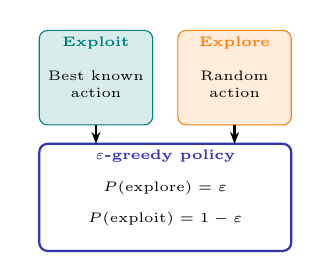
\begin{tikzpicture}[scale=0.8]
% Exploit side
\draw[dfteal, fill=dfteal!15, rounded corners=3pt] (0,2.5) rectangle (1.8,4.0);
\node[font=\tiny\bfseries, dfteal] at (0.9,3.8) {Exploit};
\node[font=\tiny, text width=1.5cm, align=center] at (0.9,3.15) {Best known action};
% Explore side
\draw[mlorange, fill=mlorange!15, rounded corners=3pt] (2.2,2.5) rectangle (4.0,4.0);
\node[font=\tiny\bfseries, mlorange] at (3.1,3.8) {Explore};
\node[font=\tiny, text width=1.5cm, align=center] at (3.1,3.15) {Random action};
% Epsilon-greedy
\draw[mlpurple, thick, rounded corners=3pt] (0,0.5) rectangle (4.0,2.2);
\node[font=\tiny\bfseries, mlpurple] at (2.0,2.0) {$\varepsilon$-greedy policy};
\node[font=\tiny] at (2.0,1.5) {$P(\text{explore}) = \varepsilon$};
\node[font=\tiny] at (2.0,1.0) {$P(\text{exploit}) = 1 - \varepsilon$};
% Arrows
\draw[-{Stealth[length=1.5mm]}, thick] (0.9,2.5) -- (0.9,2.2);
\draw[-{Stealth[length=1.5mm]}, thick] (3.1,2.5) -- (3.1,2.2);
\end{tikzpicture}
\end{columns}

\bottomnote{Multi-armed bandit: the simplest RL problem. $N$ slot machines with unknown payout distributions -- how do you maximize winnings?}
\end{frame}

%% ================================================================
%% SLIDE 5: Q-Learning
%% ================================================================
\begin{frame}[t]{Q-Learning: Estimating Future Rewards}
\begin{columns}[T]
\column{0.55\textwidth}
\small
\textbf{The Q-Value Function}
\begin{compactlist}
\item $Q(s,a)$ = expected cumulative reward from taking action $a$ in state $s$, then acting optimally
\item \highlight{Update rule} (after observing reward $r$ and next state $s'$):
\end{compactlist}

\vspace{2mm}
\footnotesize
\[Q(s,a) \leftarrow Q(s,a) + \alpha\bigl[r + \gamma \max_{a'} Q(s',a') - Q(s,a)\bigr]\]

\vspace{1mm}
\small
\begin{compactlist}
\item $\alpha$: learning rate (step size)
\item $\gamma$: discount factor (patience)
\item The term in brackets is the \highlight{temporal difference error}
\end{compactlist}

\begin{block}{Insight}
\scriptsize Q-learning is model-free: it learns the value of actions without knowing the environment's transition dynamics.
\end{block}

\column{0.42\textwidth}
\vspace{2mm}
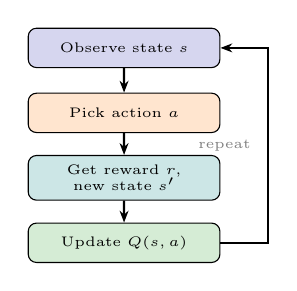
\begin{tikzpicture}[scale=0.75,
  stepnode/.style={draw, rounded corners=3pt, font=\tiny, text width=2.2cm, align=center, minimum height=0.5cm}]
\node[stepnode, fill=mllavender4] (s1) at (1.8,4.5) {Observe state $s$};
\node[stepnode, fill=mlorange!20] (s2) at (1.8,3.4) {Pick action $a$};
\node[stepnode, fill=dfteal!20] (s3) at (1.8,2.3) {Get reward $r$, new state $s'$};
\node[stepnode, fill=mlgreen!20] (s4) at (1.8,1.2) {Update $Q(s,a)$};
% Arrows
\draw[-{Stealth[length=1.5mm]}, thick] (s1) -- (s2);
\draw[-{Stealth[length=1.5mm]}, thick] (s2) -- (s3);
\draw[-{Stealth[length=1.5mm]}, thick] (s3) -- (s4);
% Loop back
\draw[-{Stealth[length=1.5mm]}, thick] (s4.east) -- ++(0.8,0) |- (s1.east);
\node[font=\tiny, mlgray] at (3.5,2.85) {repeat};
\end{tikzpicture}
\end{columns}

\bottomnote{Q-learning converges to the optimal policy given infinite exploration and a decaying learning rate (Watkins \& Dayan, 1992)}
\end{frame}

%% ================================================================
%% SLIDE 6: Q-Table Example
%% ================================================================
\begin{frame}[t]{Q-Table: A Simple Grid World Example}
\begin{columns}[T]
\column{0.55\textwidth}
\small
\textbf{Learning to Navigate}
\begin{compactlist}
\item Agent starts in a grid, goal is to reach the reward cell
\item Q-table stores values for every (state, action) pair
\item After many episodes, high Q-values form a path to the goal
\item The agent's policy: in each cell, pick the action with highest $Q$
\end{compactlist}

\begin{block}{Insight}
\scriptsize The Q-table is a lookup table -- it works for small state spaces but becomes impractical when states are continuous or high-dimensional.
\end{block}

\column{0.42\textwidth}
\vspace{2mm}
\includegraphics[width=0.55\textwidth]{04_q_learning_grid/chart.pdf}
\end{columns}

\bottomnote{A 4$\times$4 grid with 4 actions has 64 Q-values. A stock trading environment with continuous prices has infinitely many -- hence deep Q-networks.}
\end{frame}

%% ================================================================
%% SLIDE 7: Deep Q-Networks
%% ================================================================
\begin{frame}[t]{Deep Q-Networks: Scaling Up with Neural Nets}
\begin{columns}[T]
\column{0.55\textwidth}
\small
\textbf{From Table to Network}
\begin{compactlist}
\item Replace the Q-table with a neural network: $Q(s,a;\theta) \approx Q^*(s,a)$
\item Input: state $s$; output: Q-values for all actions
\item \highlight{Experience replay}: store past transitions, sample random mini-batches to break correlation
\item \highlight{Target network}: a frozen copy of $Q$ updated periodically to stabilize training
\end{compactlist}

\begin{block}{Insight}
\scriptsize DQN (Mnih et al., 2015) learned to play Atari games from raw pixels -- the same architecture can learn trading policies from price histories.
\end{block}

\column{0.42\textwidth}
\vspace{4mm}
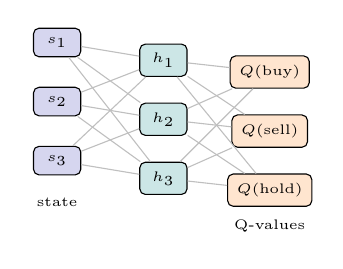
\begin{tikzpicture}[scale=0.75,
  layernode/.style={draw, rounded corners=2pt, font=\tiny, minimum width=0.6cm, minimum height=0.35cm, align=center}]
% Input layer
\node[layernode, fill=mllavender4] (i1) at (0,3.5) {$s_1$};
\node[layernode, fill=mllavender4] (i2) at (0,2.5) {$s_2$};
\node[layernode, fill=mllavender4] (i3) at (0,1.5) {$s_3$};
\node[font=\tiny] at (0,0.8) {state};
% Hidden layer
\node[layernode, fill=dfteal!20] (h1) at (1.8,3.2) {$h_1$};
\node[layernode, fill=dfteal!20] (h2) at (1.8,2.2) {$h_2$};
\node[layernode, fill=dfteal!20] (h3) at (1.8,1.2) {$h_3$};
% Output layer
\node[layernode, fill=mlorange!20] (o1) at (3.6,3.0) {$Q(\text{buy})$};
\node[layernode, fill=mlorange!20] (o2) at (3.6,2.0) {$Q(\text{sell})$};
\node[layernode, fill=mlorange!20] (o3) at (3.6,1.0) {$Q(\text{hold})$};
% Connections
\foreach \i in {i1,i2,i3} {
  \foreach \h in {h1,h2,h3} {
    \draw[mlgray!50, thin] (\i) -- (\h);
  }
}
\foreach \h in {h1,h2,h3} {
  \foreach \o in {o1,o2,o3} {
    \draw[mlgray!50, thin] (\h) -- (\o);
  }
}
\node[font=\tiny] at (3.6,0.4) {Q-values};
\end{tikzpicture}
\end{columns}

\bottomnote{Experience replay and target networks were the two key innovations that made deep RL stable enough to work in practice}
\end{frame}

%% ================================================================
%% SLIDE 8: Reward Design
%% ================================================================
\begin{frame}[t]{Reward Design: Shaping the Objective}
\begin{columns}[T]
\column{0.55\textwidth}
\small
\textbf{The Reward Is Everything}
\begin{compactlist}
\item The agent optimizes exactly what you reward -- nothing more, nothing less
\item \highlight{Sparse rewards}: only signal at episode end (e.g., final PnL). Hard to learn from.
\item \highlight{Shaped rewards}: intermediate signals (e.g., Sharpe ratio per step). Faster learning but risk of reward hacking.
\item \highlight{Credit assignment}: which past action caused today's reward? Delayed rewards make learning harder.
\end{compactlist}

\begin{block}{Insight}
\scriptsize Reward design is the hardest part of RL. A badly designed reward function produces an agent that ``cheats'' -- technically optimal but practically useless.
\end{block}

\column{0.42\textwidth}
\vspace{2mm}
\footnotesize
\fcolorbox{mlpurple}{mllavender4}{\parbox{0.85\columnwidth}{%
\textbf{Trading Reward Examples:}

\vspace{2mm}
\textcolor{dfred}{Naive}: $r_t = \text{PnL}_t$

$\rightarrow$ Agent takes maximum leverage

\vspace{2mm}
\textcolor{dfteal}{Better}: $r_t = \frac{\text{PnL}_t}{\sigma_t}$ (Sharpe)

$\rightarrow$ Balances return and risk

\vspace{2mm}
\textcolor{mlgreen}{With constraint}: penalize drawdown

$r_t = \text{Sharpe}_t - \lambda \cdot \text{DD}_t$
}}
\end{columns}

\bottomnote{Goodhart's Law: ``When a measure becomes a target, it ceases to be a good measure'' -- applies directly to RL reward design}
\end{frame}

%% ================================================================
%% SLIDE 9: Finance Application
%% ================================================================
\begin{frame}[t]{Finance Application: Algorithmic Trading with RL}
\begin{columns}[T]
\column{0.55\textwidth}
\small
\textbf{RL for Portfolio Management}
\begin{compactlist}
\item \highlight{States}: price history, technical indicators, portfolio positions, market regime
\item \highlight{Actions}: buy, sell, hold (or continuous: allocation weights)
\item \highlight{Reward}: risk-adjusted return (Sharpe ratio, Sortino ratio)
\item Agent learns when to enter/exit positions without explicit rules
\end{compactlist}

\begin{block}{Insight}
\scriptsize RL is not widely deployed in live trading yet -- simulation-to-reality gap, non-stationarity, and reward design remain open challenges.
\end{block}

\column{0.42\textwidth}
\vspace{2mm}
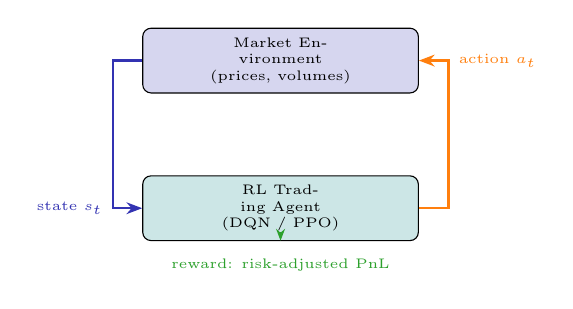
\begin{tikzpicture}[scale=0.75,
  mnode/.style={draw, rounded corners=3pt, font=\tiny, text width=1.8cm, align=center, minimum height=0.5cm}]
% Market (environment)
\node[mnode, fill=mllavender4, minimum width=3.5cm] (mkt) at (2.0,4.0) {Market Environment\\(prices, volumes)};
% Agent
\node[mnode, fill=dfteal!20, minimum width=3.5cm] (agent) at (2.0,1.5) {RL Trading Agent\\(DQN / PPO)};
% State arrow
\draw[-{Stealth[length=2mm]}, thick, mlpurple] (mkt.west) -- ++(-0.5,0) |- (agent.west) node[midway, left, font=\tiny] {state $s_t$};
% Action arrow
\draw[-{Stealth[length=2mm]}, thick, mlorange] (agent.east) -- ++(0.5,0) |- (mkt.east) node[midway, right, font=\tiny] {action $a_t$};
% Reward
\node[font=\tiny, mlgreen, below] at (2.0,0.8) {reward: risk-adjusted PnL};
\draw[-{Stealth[length=1.5mm]}, mlgreen, thick] (2.0,1.1) -- (2.0,0.95);
\end{tikzpicture}
\end{columns}

\bottomnote{JPMorgan's LOXM uses RL for optimal trade execution; other firms explore RL for market making and portfolio rebalancing}
\end{frame}

%% ================================================================
%% SLIDE 10: Summary
%% ================================================================
\begin{frame}[t]{Summary: Reinforcement Learning in 4 Takeaways}
\begin{columns}[T]
\column{0.95\textwidth}
\small
\begin{enumerate}
\setlength{\itemsep}{6pt}
\item \highlight{Framework}: Agent observes state, takes action, receives reward. Goal: maximize cumulative discounted reward $\sum \gamma^t r_t$.
\item \highlight{Exploration}: $\varepsilon$-greedy balances trying new actions (explore) with choosing the best known action (exploit). Start high, decay over time.
\item \highlight{Q-Learning}: Learn $Q(s,a)$ via temporal difference updates. Q-tables work for small spaces; DQN scales to complex environments.
\item \highlight{Finance}: RL enables data-driven trading, but reward design, non-stationarity, and the simulation-to-reality gap remain open challenges.
\end{enumerate}

\vspace{4mm}
\begin{block}{Next Steps}
\scriptsize Explore the deep dive slides for policy gradient methods, actor-critic architectures, and multi-agent RL. Try the notebook to train a Q-learning agent on a simulated trading environment.
\end{block}
\end{columns}

\bottomnote{RL is the most ambitious ML paradigm: learn behavior from interaction, not from labels. Finance is a natural but challenging domain.}
\end{frame}

\end{document}
